%! TEX root = **/000-main.tex
% vim: spell spelllang=en:

\section{Ontology}%
\label{sec:ontology}

\subsection{TBOX definition}%
\label{sub:tbox}

% B1. TBOX definition
% ===================
% In case you used any other tool, include a graphical representation in the pdf
% file (e.g., using https://gra.fo/) and include the rdf, rdfs or owl file
% generated by the tool in the zip file to upload and following the naming
% notation explained (IMPORTANT: the lecturer should not install any additional
% tool to validate this part).

To do the \texttt{TBOX}, we used a combination of \href{https://protege.stanford.edu/}{Protégé} and
\href{https://gra.fo}{gra.fo}. The initial design was done by hand, then translated to \emph{Protégé} where
we added different restrictions, and finally we imported it into gra.fo to visualize it.
\Cref{fig:tbox_diagram} shows the simplified TBOX diagram as rendered by gra.fo. The dotted arrows represent
\texttt{rdfs:subClassOf} relationships and the other represent the different properties (all of
them with \texttt{domain} and \texttt{range}).  We omitted some relationships we used for the restrictions
as well as the attributes in favour of clarity.

\begin{figure}[H]
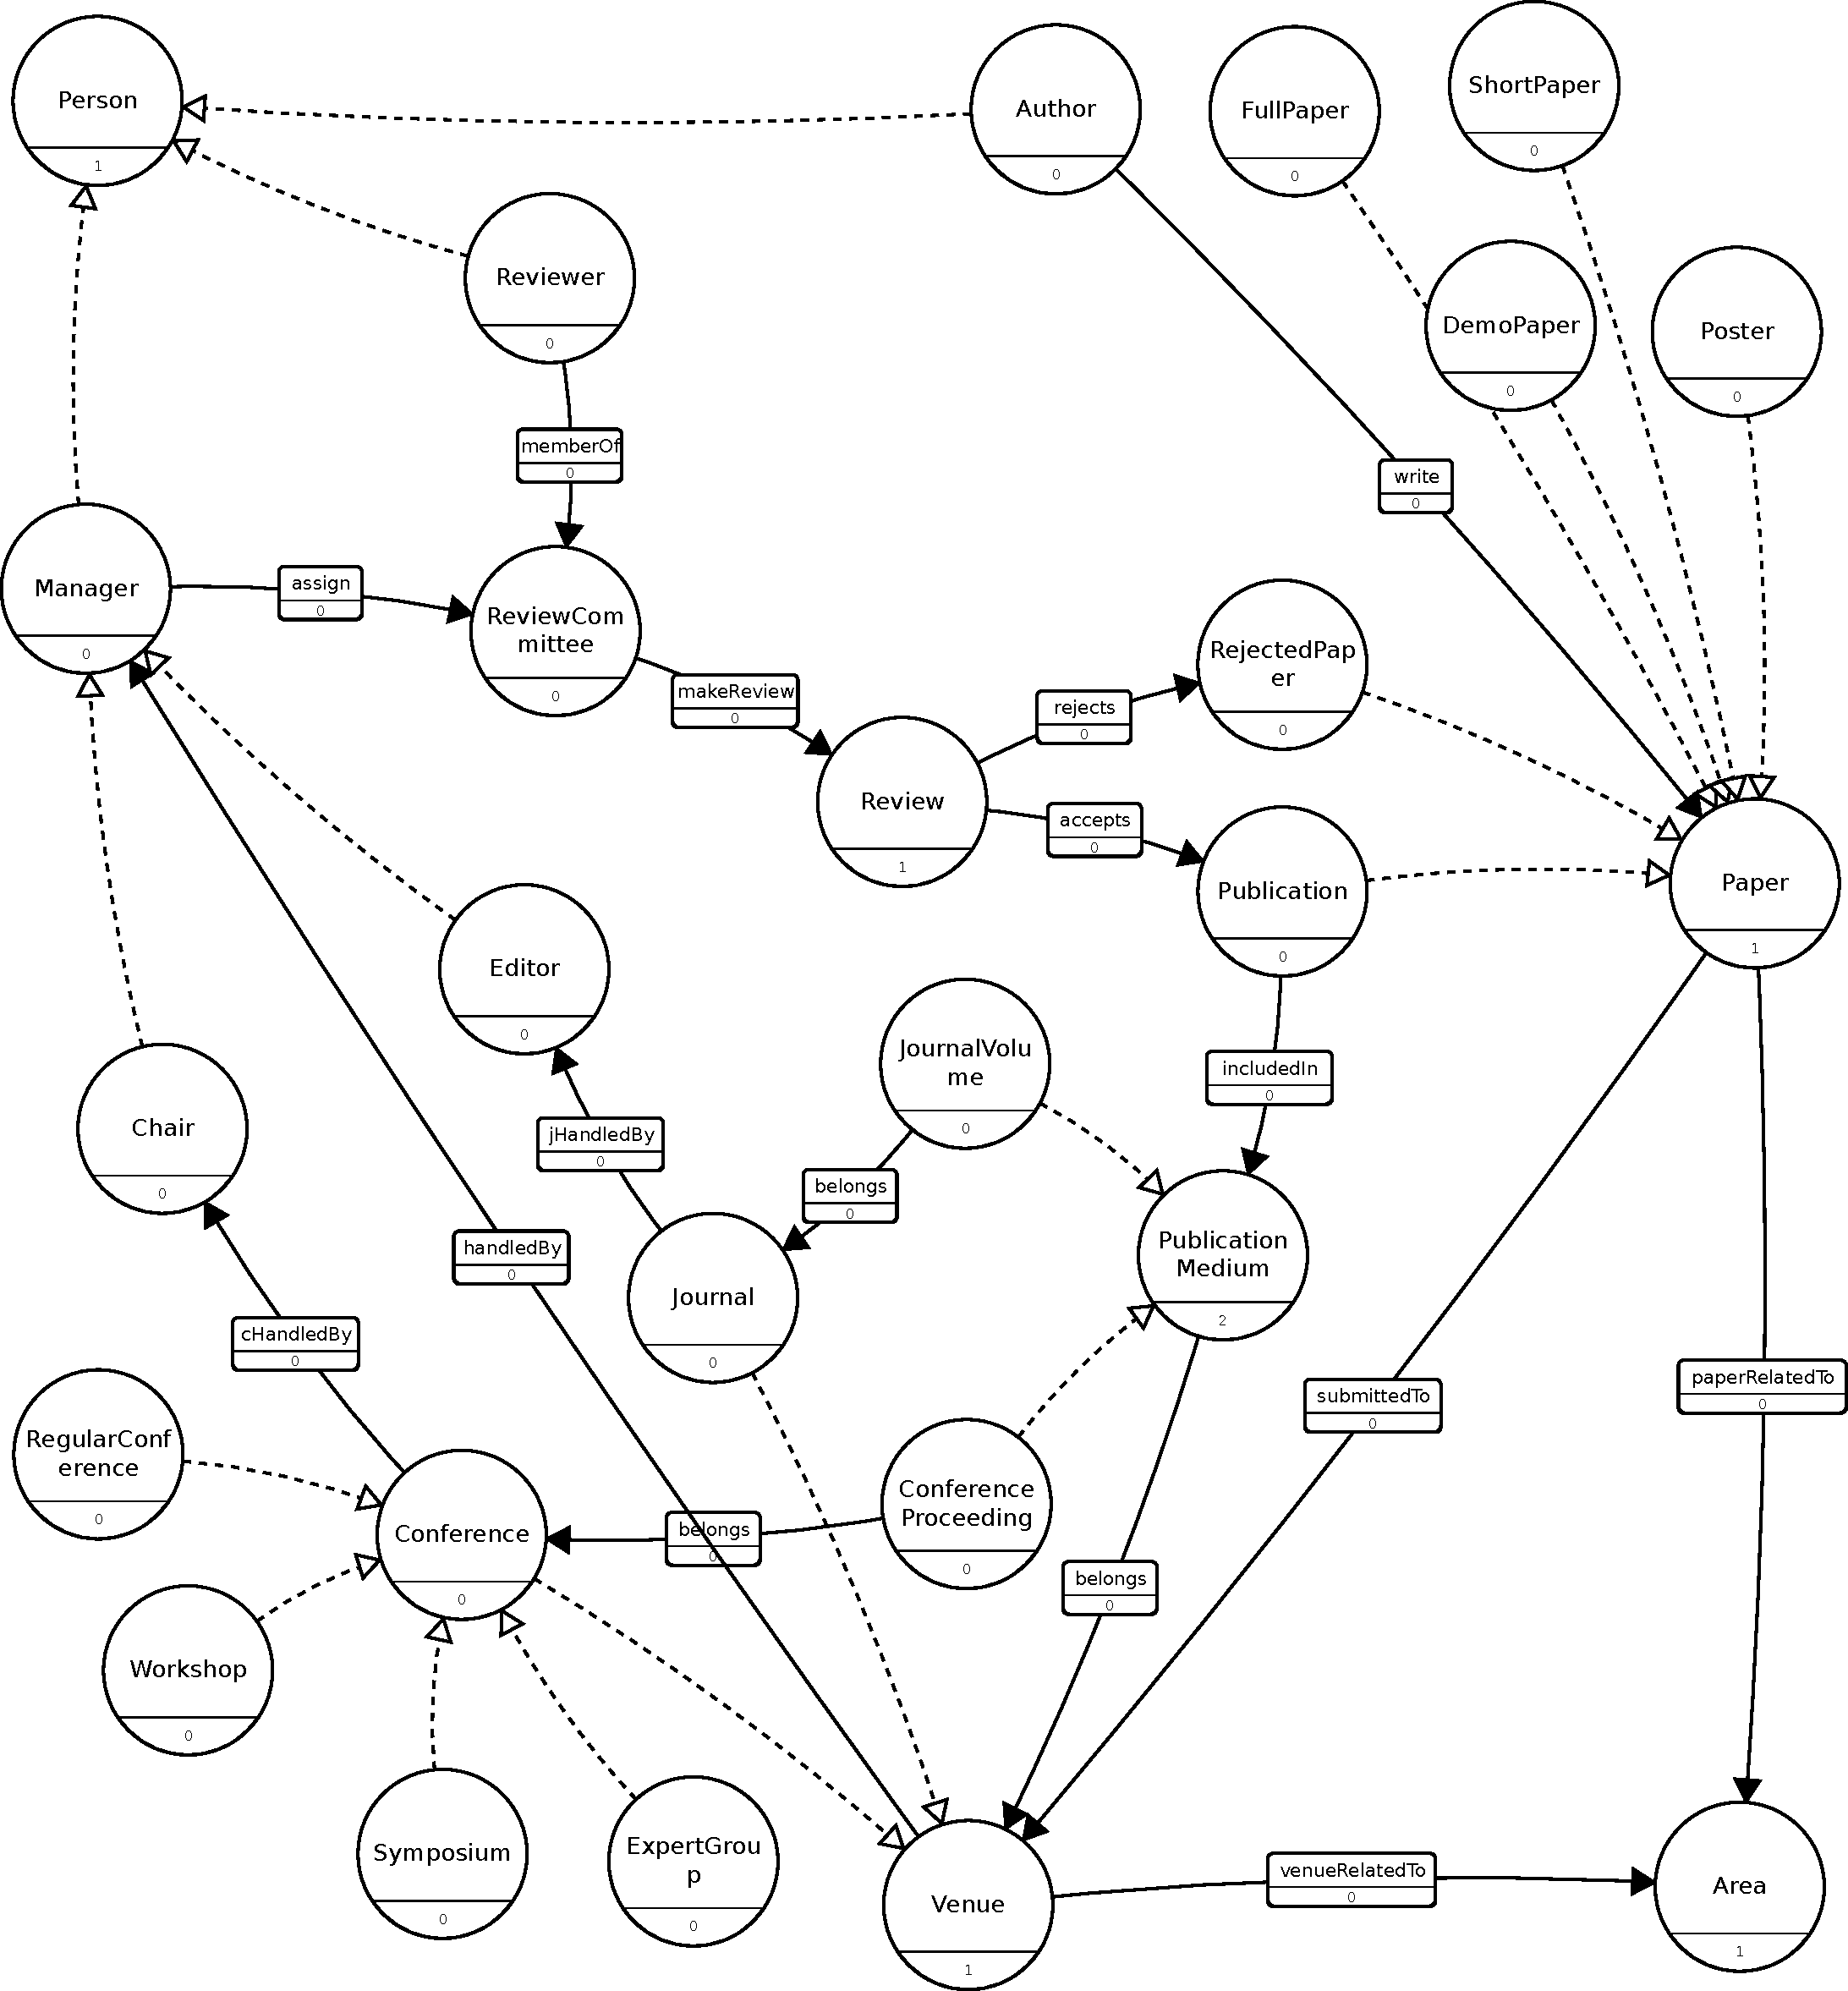
\includegraphics{sdm_lab_diagram_bw}
\caption{TBOX diagram generated using \url{gra.fo}}%
\label{fig:tbox_diagram}
\end{figure}

\pagebreak
The complete \texttt{owl} file with all the TBOX and the restrictions is included in the
zip file. The relationships not shown in the diagram are:
\begin{itemize}
\item \texttt{Poster} \rightarrow \texttt{[posterSubmittedTo]}\rightarrow \texttt{Journal} which has
    restriction: owl:maxCardinality=0. To ensure that Posters are only submitted to Conferences.
\item \texttt{Review} \rightarrow \texttt{[givesVerdict]}\rightarrow \texttt{Paper} which is
    a \emph{superProperty} of both \texttt{rejects} and \texttt{accepts}.
\item \texttt{owl:minCardinality}=2 on \texttt{memberOf} so that \texttt{ReviewCommittees} are at least
    2 members.
\end{itemize}

\pagebreak
\subsection{ABOX definition}%
\label{sub:abox}

% B2. ABOX definition
% ===================
% - In the main pdf file, explain the methodology used to define your ABOX from
%   non-semantic data.
% - In the zip file, include your code to create the ABOX programmatically
%   (e.g., Jena or RDFLib code) and the resulting ABOX file (rdf, rdfs or owl).
%   These files must follow the naming notation explained.

To generate the ABOX, we used the data we obtained in the first laboratory session
for the Neo4j and implemented a Java application that read those CSV files and generated
the final RDFS using Jena.

Our program works in the same fashion that \texttt{neo4j-admin import} worked, that
is: it has to be run from the command line and accepts various arguments which
define both the location of the file and whether it is a class (node) or a property (edge)
and how this have to be labelled in rdf. 

The arguments below show the syntax to indicate that Poster data has to be imported from
the file \texttt{papers\_a.csv} in folder \texttt{\$DATA} and the relationship \texttt{writes}
between \texttt{Author} and \texttt{Paper} is defined in \texttt{rel\_writes.csv}.

\begin{minted}{bash}
    --node="Paper:Poster=${DATA}/papers_a.csv" \
    --node="Paper:DemoPaper=${DATA}/papers_b.csv" \
    --node="Paper:FullPaper=${DATA}/papers_c.csv" \
    --node="Paper:ShortPaper=${DATA}/papers_d.csv" \
    --node="Author=${DATA}/authors.csv" \
    --edge="write=Author=Paper=${DATA}/rel_writes.csv"
\end{minted}

All the csv files data as well as the script with the required arguments to generate
our ABOX are provided in the delivery zip file. The original program that was developed
for laboratory 1, and we used to obtain the zip files is publicly available at:
\href{https://github.com/Leixb/Aminer-citations-to-csv-for-neo4j/tree/sdm-lab3}{Leixb/Aminer-citations-to-csv-for-neo4j}\footnote{Some modifications were made in order to collect different data, since the required data differed slightly from session 1}

\pagebreak
\subsection{Inference regime}%
\label{sub:inference}

We used RDFS inference regime entailment with the subclasses shown in the previous section. Therefore,
we saved the most specific definitions on our
data, for instance, for Venues we saved Workshop, RegularConference, ExperGroup, Symposium and Journal
which through inference will all be also of type Venue (all but the later are also inferred to be Conference)

% B3. Create the final ontology
% =============================
% Besides that, you need to provide two additional outputs for this section
% (both must be included in the main pdf file of the deliverable):
% - Specify the inference regime entailment you are considering. Briefly explain
%   what rdf:type links you saved to explicitly generate thanks to reasoning.
% - Provide a summary table of your instances. Compute simple statistics about
%   the resulting knowledge graph. For example, the number of classes, the
%   number of properties, number of instances for the main classes and number of
%   triples using the main properties.

\begin{table}[H]
\centering
\caption{Summary of instances}
\label{tab:summary_instances}
\begin{tabular}{lr}
  \toprule
  Property & Value \\
  \midrule
  Number of classes & 25\\
  Number of properties & 20\\
  Number of instances of "Person" class & 15,276\\
  Number of instances of "Paper" class & 9,999\\
  Number of instances of "Venue" class & 9,200\\
  Number of triples using "write" property & 17,388\\
  Number of triples using "includedIn" property & 9,999\\
    Number of triples using "makeReview" property & 31,274\\
  \bottomrule
\end{tabular}
\end{table}

The table 1 summarizes the instances of our resulting knowledge graph. These numbers were found thanks to the SPARQL queries below: 
\begin{enumerate}
\item Number of classes.
\begin{minted}{sparql}
PREFIX owl: <http://www.w3.org/2002/07/owl#>

SELECT ?class 
WHERE {?class a owl:Class}
\end{minted}
\item Number of properties.
\begin{minted}{sparql}
PREFIX owl: <http://www.w3.org/2002/07/owl#>

SELECT ?property 
WHERE {
   {?property a owl:DatatypeProperty}
     UNION
   {?property a owl:ObjectProperty}
}
\end{minted}
\item Number of instances for the main classes (Author).
\begin{minted}{sparql}
PREFIX sdm: <http://www.semanticweb.org/emmasalvan/ontologies/2022/4/sdmlab3#>
PREFIX rdf: <http://www.w3.org/1999/02/22-rdf-syntax-ns#>

SELECT ?c
WHERE {?c rdf:type sdm:Author}
\end{minted}
\item Number of triples for the main properties (write).
\begin{minted}{sparql}
PREFIX sdm: <http://www.semanticweb.org/emmasalvan/ontologies/2022/4/sdmlab3#>

SELECT ?d ?r
WHERE {?d sdm:write ?r}
\end{minted}
\end{enumerate}

\begin{table}[H]
\centering
\caption{Summary of classes}
\label{tab:summary}
\begin{tabular}{lr}
  \toprule
  Class\\
  \midrule
  :Area\\
  :Author\\
  :Chair\\
  :Conference\\
  :ConferenceProceeding\\
  :DemoPaper\\
  :Editor\\
  :ExpertGroup\\
  :FullPaper\\
  :Journal\\
  :JournalVolume\\
  :Manager\\
  :Paper\\
  :Person\\
  :Poster\\
  :Publication\\
  :PublicationMedium\\
  :RegularConference\\
  :RejectedPaper\\
  :Review\\
  :Reviewer\\
  :ReviewCommitte\\
  :ShortPaper\\
  :Symposium\\
  :Venue\\
  :Workshop\\
  \bottomrule
\end{tabular}
\end{table}

\pagebreak
\subsection{Querying the ontology}%
\label{sub:querying}

% B4. Querying the ontology
% =========================
% In the main pdf file, provide the following SPARQL queries (explicitly state
% any assumption you make):
% - Find all Authors.
% - Find all properties whose domain is Author.
% - Find all properties whose domain is either Conference or Journal.
% - Find all the papers written by a given author that where published in
%   database conferences.

\begin{enumerate}
\item Find all Authors.
\begin{minted}{sparql}
PREFIX sdm: <http://www.semanticweb.org/emmasalvan/ontologies/2022/4/sdmlab3#>

SELECT ?authorName
WHERE {?Author sdm:pName ?authorName}
\end{minted}
\item Find all properties whose domain is Author.
\begin{minted}{sparql}
PREFIX sdm: <http://www.semanticweb.org/emmasalvan/ontologies/2022/4/sdmlab3#>
PREFIX rdfs: <http://www.w3.org/2000/01/rdf-schema#>

SELECT DISTINCT ?property
WHERE {?property rdfs:domain sdm:Author}
\end{minted}
\item Find all properties whose domain is either Conference or Journal.
\begin{minted}{sparql}
PREFIX sdm: <http://www.semanticweb.org/emmasalvan/ontologies/2022/4/sdmlab3#>
PREFIX rdfs: <http://www.w3.org/2000/01/rdf-schema#>

SELECT DISTINCT ?property
WHERE {
    {?property rdfs:domain sdm:Conference}
        UNION 
    {?property rdfs:domain sdm:Journal}
}
\end{minted}
\item Find all the papers written by a given author that were published in database conferences.
\begin{minted}{sparql}
PREFIX sdm: <http://www.semanticweb.org/emmasalvan/ontologies/2022/4/sdmlab3#>
PREFIX rdf: <http://www.w3.org/1999/02/22-rdf-syntax-ns#>
PREFIX rdfs: <http://www.w3.org/2000/01/rdf-schema#>

SELECT ?paperTitle ?paper ?conference ?proceedings
WHERE {
    sdm:Author-15156 sdm:write ?paper .
    ?paper sdm:includedIn ?proceedings .
    ?proceedings a sdm:ConferenceProceeding .
    ?proceedings sdm:belongs ?conference .
    ?conference sdm:venueRelatedTo ?area .
    ?area sdm:aName "Database" .
    ?paper sdm:title ?paperTitle
}
\end{minted}
\end{enumerate}


